\section*{Chapter 2: Overview of supervised learning}

\subsection*{Ex. 2.1}
Since $||t_k||^2 = 1$, one has:
\begin{eqnarray}
||t_k - \hat{y}||^2 = 1 - 2 \hat{y}_k + ||\hat{y}||^2
\end{eqnarray}
hence:
\begin{eqnarray}
\textrm{argmin}_k ||t_k - \hat{y}|| = \textrm{argmin}_k ||t_k - \hat{y}||^2 = 
\textrm{argmax}_k\, \hat{y}_k
\end{eqnarray}

\subsection*{Ex. 2.2}
This assignment is slightly ambiguous, since the  we are told that the 100 examples 
are generated for each class but the \textit{a priori} probabilities $P(Y = \pm 1)$
are not specified. We interpret the exercise as $P(Y = \pm 1) = 1/2$, and obtain the 
probability distribution:
\begin{eqnarray}
P(Y = \pm 1) & = & \frac{1}{2} \\
P(x | Y = \pm 1) & = & \frac{1}{10} \sum_{k=1}^{10} \mathcal{N}(x ; m_k ^{\pm}, \mathbb{I} / 5)
\end{eqnarray}
The decision boundary is the set points $x$ for which:
\begin{eqnarray}
P(Y = +1 |X = x) = P(Y = -1| X = x)
\end{eqnarray}
From Bayes theorem and the fact that $P(Y = +1) = P(Y =-1)$, this is equivalent to:
\begin{eqnarray}
p(x|Y = +1) = p(x|Y = -1)
\end{eqnarray}
which upon simplification reads:
\begin{eqnarray}
\sum_{k=1}^{10} \exp \left( 5\,m_k ^{+ T} x - \frac{5}{2} m_k ^{+ T} m_k^+ \right) = 
\sum_{k=1}^{10} \exp \left( 5\,m_k ^{- T} x - \frac{5}{2} m_k ^{- T} m_k^- \right)
\end{eqnarray}
Note how with one gaussian per class instead of 10 the decision boundary becomes 
linear (LDA).

\subsection*{Ex. 2.3}

The variables $\rho_i \equiv ||x_i||$ are i.i.d. with c.d.f.: 
\begin{eqnarray}
P(\rho_i \leq \bar{\rho}) = \bar{\rho}^p
\end{eqnarray}
So letting $\rho_m \equiv \min(\{\rho_i\}_{i=1,\ldots,N})$, one has:
\begin{eqnarray}\label{eq:2p3_1}
P\left(\rho_m \geq \bar{\rho}\right) = \prod_{i=1}^{N}P\left(\rho_i \geq 
\bar{\rho}\right) = \left(1 - \rho^p \right)^N
\end{eqnarray}
The median of $\rho_m$ is the value $\rho^\star$ s.t. $P\left(\rho_m \geq 
\rho^\star\right) = 1/2$. Using \eqref{eq:2p3_1} it is easy to see that:
\begin{eqnarray}
\rho^\star = \left(1 - \frac{1}{2^{1/N}} \right) ^{1/p}
\end{eqnarray}

\subsection*{Ex. 2.4}

The components $(X_j)_{j=1,\ldots,p}$ of $X$ are i.i.d. centered and unit variance 
gaussians. Hence, the linear combination $Z \equiv a^T X$ is still gaussian and 
centered, and its variance is also one:
\begin{eqnarray}
\textrm{Var}\left(\sum_{j=1}^p a_j X_j \right) = \sum_{j=1}^p a_j^2 = 1
\end{eqnarray}

\subsection*{Ex. 2.5}

The random variables $y_0$ and $\hat{y}_0$ are independent, hence:
\begin{eqnarray*}
\textrm{EPE}(x_0) & \equiv & \mathbb{E}_{\mathcal{T}, y_0|x_0} \left[ (y_0 - \hat{y}_0)^2 \right] = \left( \mathbb{E}_{\mathcal{T}, y_0|x_0} \left[ y_0 - \hat{y}_0 \right] \right) ^2 + \textrm{Var}_{\mathcal{T}, y_0|x_0} \left( y_0 - \hat{y}_0 \right) \\
& = & \left( \mathbb{E}_{y_0 | x_0}\left[y_0\right] - \mathbb{E}_{\mathcal{T}}\left[\hat{y}_0 \right] \right)^2 + \textrm{Var}_{y_0 | x_0} (y_0) + \textrm{Var}_{\mathcal{T}}(\hat{y}_0) 
\end{eqnarray*}
We obtain the decomposition of expected prediction error as a sum of irreducible variance, squared bias and estimation variance:
\begin{eqnarray}
\textrm{EPE}(x_0) & = & \textrm{Var}_{y_0 | x_0} (y_0) + \textrm{Bias}_{\mathcal{T}, y_0 | x_0}^2(y_0) + \textrm{Var}_\mathcal{T}(\hat{y}_0)\\
\textrm{Var}_{y_0 | x_0} (y_0) & \equiv & \mathbb{E}_{y_0 | x_0}\left[\left(y_0 - \mathbb{E}_{y_0 | x_0}\left[y_0\right]\right)^2 \right]\\
\textrm{Bias}_{\mathcal{T}, y_0 | x_0}(y_0) & \equiv & \mathbb{E}_{y_0 | x_0}\left[y_0\right] - \mathbb{E}_{\mathcal{T}}\left[\hat{y}_0 \right] \\
\textrm{Var}_\mathcal{T}(\hat{y}_0) & \equiv & \mathbb{E}_{\mathcal{T}}\left[\left(\mathbb{E}_{\mathcal{T}}\left[\hat{y}_0 \right] - \hat{y}_0 \right)^2 \right]
\end{eqnarray}
Equation (2.27) was obtained under two assumptions:
\begin{itemize}
	\item the underlying distribution for $Y$ conditional on $X$ is:
	$$
	y = \beta ^T X + \epsilon, \quad \epsilon \sim \mathcal{N}(0, \sigma^2)
	$$
	from which it follows that:
	\begin{eqnarray*}
		\mathbb{E}_{y_0 | x_0}\left[y_0\right] & = & \beta ^T x_0\\
		\textrm{Var}_{y_0 | x_0} (y_0) & = & \sigma^2
	\end{eqnarray*}
	\item $\hat{y}_0$ is an OLS estimate of $Y$ at $X = x_0$:
	$$
	\hat{y}_0 = x_0 ^T \left(\mathbf{X}^T \mathbf{X} \right)^{-1} \mathbf{X}^T \left(\mathbf{X} \beta + \bm{\epsilon}\right) = x_0 ^T \beta + x_0^T \left(\mathbf{X}^T \mathbf{X} \right)^{-1} \mathbf{X}^T \bm{\epsilon}
	$$
\end{itemize}
By assumption $\epsilon$ and $X$ are independent random variables. Hence, denoting $p_X \equiv \mathbf{X} \left( \mathbf{X}^T \mathbf{X} \right)^{-1} x_0$ such that $\hat{y}_0 = x_0^T \beta + p_X^T \bm{\epsilon}$, one has:
\begin{eqnarray*}
	\mathbb{E}_{\mathcal{T}} \left[ p_X^T\, \epsilon\right] & = & \mathbb{E}_\mathbf{X}
	\left[p_X^T\right]\, \mathbb{E}_\epsilon \left[\bm{\epsilon}\right] \\
	\mathbb{E}_{\mathcal{T}}\left[\hat{y}_0 \right] & = & x_0 ^T \beta\\
	\textrm{Var}_\mathcal{T}(\hat{y}_0) & = & \mathbb{E}_{\mathcal{T}}\left[ (p_X^T \bm{\epsilon})^2\right] = \mathbb{E} _\mathcal{T}\left[p_X^T \bm{\epsilon} \, \bm{\epsilon}^T p_X \right] = \mathbb{E} _\mathcal{T}\left[\textrm{Tr} \left(p_X^T \bm{\epsilon} \, \bm{\epsilon}^T p_X \right)\right]\\
	& = & \mathbb{E} _\mathcal{T}\left[\textrm{Tr} \left(p_X\, p_X^T \bm{\epsilon} \, \bm{\epsilon}^T \right)\right] \\
	& = & \textrm{Tr} \left(	
	\mathbb{E}_\mathbf{X} \left[ p_X p_X^T \right] \mathbb{E}_{\bm{\epsilon}} \left[\bm{\epsilon} \bm{\epsilon}^T \right]\right) = \sigma ^2 \mathbb{E}_\mathbf{X} \left[x_0^T (\mathbf{X}^T \mathbf{X})^{-1} x_0 \right]
\end{eqnarray*}
The last equality follows from the cyclicity and linearity of trace. Using 
$\mathbb{E}_{\bm{\epsilon}} \left[\bm{\epsilon} \bm{\epsilon}^T \right] = \sigma^2$ one
has:
\begin{eqnarray*}
\textrm{Var}_\mathcal{T}(\hat{y}_0) & = & \sigma^2 \,\textrm{Tr} \left(	
	\mathbb{E}_\mathbf{X} \left[ p_X p_X^T \right] \right) \\
& = & \sigma^2 \, \mathbb{E}_\mathbf{X} \left[ \textrm{Tr}\left(p_X p_X^T \right)\right] 
 	= \sigma^2 \, \mathbb{E}_\mathbf{X} \left[ ||p_X||^2 \right]\\
& = & \sigma ^2 \mathbb{E}_\mathbf{X} \left[x_0^T (\mathbf{X}^T \mathbf{X})^{-1} x_0 
	\right]
\end{eqnarray*}
Putting everything together:
\begin{eqnarray*}
\textrm{Var}_{y_0 | x_0} (y_0) & = & \sigma^2\\
\textrm{Bias}_{\mathcal{T}, y_0 | x_0}(y_0) & = & 0\\
\textrm{Var}_\mathcal{T}(\hat{y}_0) & = & \sigma ^2\, \mathbb{E}_\mathbf{X} \left[x_0^T 
	(\mathbf{X}^T \mathbf{X})^{-1} x_0 \right]\\
\textrm{EPE}(x_0) & = & \sigma^2\, \left( 1 + \mathbb{E}_\mathbf{X} \left[x_0^T 
	(\mathbf{X}^T \mathbf{X})^{-1} x_0 \right] \right)
\end{eqnarray*} 
which proves Eq. (2.27).

To prove Eq. (2.28) under the specified assumption:
$$
(\mathbf{X}^T \mathbf{X})^{-1} \rightarrow N^{-1} \textrm{Cov}^{-1}(X) \quad \textrm{as} \; N \rightarrow \infty
$$
requires a simple manipulation involving the cyclicity and linearity of the trace operation, as well as the independence of $\mathbf{X}$ and $x_0$:
\begin{eqnarray*}
\mathbb{E}_{x_0} \left[EPE(x_0) \right] & = &\sigma^2 \left(1 + \mathbb{E}_{x_0, 
    \mathbf{X}} \left[x_0^T (\mathbf{X}^T \mathbf{X})^{-1} x_0\right] \right) \\
& = &\sigma^2 \left(1 + \mathbb{E}_{x_0, \mathbf{X}} \left[\textrm{Tr}\left(x_0^T 
    (\mathbf{X}^T \mathbf{X})^{-1} x_0 \right)\right] \right) \\
& = &\sigma^2 \left(1 + \mathbb{E}_{x_0, \mathbf{X}} \left[\textrm{Tr}\left(x_0 x_0^T 
    (\mathbf{X}^T \mathbf{X})^{-1} \right)\right] \right)\\
& = &\sigma^2 \left(1 + \textrm{Tr}\left(\mathbb{E}_{x_0, \mathbf{X}} \left[x_0 x_0^T 
    (\mathbf{X}^T \mathbf{X})^{-1} \right]\right) \right)\\
& = &\sigma^2 \left(1 + \textrm{Tr}\left(\mathbb{E}_{x_0} \left[x_0 x_0^T \right] 
    \mathbb{E}_{\mathbf{X}}\left[ (\mathbf{X}^T \mathbf{X})^{-1} \right]\right) \right)\\
& = &\sigma^2 \left(1 + \textrm{Tr}\left(\textrm{Cov}(x_0)\, 
    \mathbb{E}_{\mathbf{X}}\left[ (\mathbf{X}^T \mathbf{X})^{-1} \right]\right) \right)\\
& \rightarrow &\sigma^2 \left(1 + \frac{1}{N} \textrm{Tr}\left(\textrm{Cov}(x_0)\, 
    \textrm{Cov}^{-1}(X)\right) \right)\\
& = & \sigma^2 \left(1 + \frac{p}{N} \right)
\end{eqnarray*}
The last equality follows from the fact that $x_0$ is drawn from the same distribution 
as $X$. 


\subsection*{Ex. 2.6}

One has:
$$
\sum_{i:\, x_i = x} \left(y_i - f_\theta(x_i) \right)^2 = n_x \left(\bar{y}_x - 
	f_\theta(x)\right)^2 + \sum_{i:\, x_i = x} \left(y_i - \bar{y}_x \right)^2
$$
where $n_x \equiv \sum_{i:\, x_i = x} 1$ and $\bar{y}_x \equiv n_x^{-1} \sum_{i:\, x_i = 
x} y_i$. The second term does not contribute to the regression since it does not depend 
on $f_\theta$, so we can just fit using the average $\bar{y}_x$ as response and weights 
proportional to $n_x$.

\subsection*{Ex. 2.7}

\subsubsection*{Point (a)}

One has:
\begin{eqnarray*}
\textrm{linear regression:} \quad && \hat{f}(x_0) = x_0^T \hat{\beta} = x_0^T (\mathbf{X} ^{T} \mathbf{X}) ^{-1} \mathbf{X} ^{T} Y \\
     && l_i(x_0, \mathcal{X}) = \left( \mathbf{X} (\mathbf{X} ^{T}\mathbf{X}) ^{-1} x_0\right)_i \\
\textrm{k-nn:} \quad && l_i(x_0, \mathcal{X}) = \frac{1}{k}\, \mathbf{I} \left( x_i \textrm{ is among the } k \textrm{ closest neighbors of } x_0 \right)
\end{eqnarray*}

\subsubsection*{Point (b)}

Notice that:
\begin{eqnarray*}
\mathbb{E}_{\mathcal{Y}|\mathcal{X}} \left[ \hat{f}(x_0) \right] & = & \bm{l}^{T}(x_0; \mathcal{X})\,\bm{f}(X),\\
\textrm{Var}_{\mathcal{Y}|\mathcal{X}}\left( \hat{f}(x_0) \right) & = & \bm{l}^{T}(x_0; \mathcal{X})\, \textrm{Cov}(\bm{\epsilon}) \, \bm{l}(x_0; \mathcal{X}) = \sigma^2 \, ||\bm{l}(x_0; \mathcal{X})||^2
\end{eqnarray*}
where we denoted $(\bm{l}(x_0; \mathcal{X}))_i \equiv l_i(x_0; \mathcal{X})$ and $(\bm{f}(X))_i \equiv f(x_i)$. Hence:
\begin{eqnarray*}
\mathbb{E}_{\mathcal{Y}| \mathcal{X}} \left[ \left( f(x_0) - \hat{f}(x_0) \right)^2 \right]  & = & \textrm{Bias}^2_{\mathcal{Y}| \mathcal{X}}(y_0) + \textrm{Var}_{\mathcal{Y}| \mathcal{X}}(y_0)\\ 
\textrm{Bias}^2_{\mathcal{Y}| \mathcal{X}}(y_0) & \equiv & \left( f(x_0) - \bm{l}^{T}(x_0; \mathcal{X})\,\bm{f}(X) \right)^2\\
\textrm{Var}_{\mathcal{Y}| \mathcal{X}}(y_0) & \equiv & \sigma^2 ||\bm{l}(x_0; \mathcal{X})||^2 
\end{eqnarray*}
The first term represents the bias, while the second represents the variance of the estimator as the training responses vary for fixed $\mathcal{X}$.

\subsubsection*{Point (c)}

For this part can go down a similar road, using now the independence of $X$ and $\epsilon$:
\begin{eqnarray*}
\mathbb{E}_{\mathcal{Y},\mathcal{X}} \left[ \hat{f}(x_0) \right] & = & \mathbb{E}_{\mathcal{X}} \left[ \bm{l}^T(x_0; \mathcal{X}) \, \bm{f}(X) \right],\\
\textrm{Var}_{\mathcal{Y},\mathcal{X}}\left( \hat{f}(x_0) \right) & = & \textrm{Var}_{\mathcal{X}} \left( \bm{l}^T(x_0; \mathcal{X}) \, \bm{f}(X) \right) + 
\sigma ^2 \mathbb{E}_{\mathcal{X}} \left[ ||\bm{l}(x_0; \mathcal{X})||^2  \right],
\end{eqnarray*}
Hence:
\begin{eqnarray*}
\mathbb{E}_{\mathcal{Y}, \mathcal{X}} \left[ \left( f(x_0) - \hat{f}(x_0) \right)^2 \right] & = & \textrm{Bias}^2_{\mathcal{Y}, \mathcal{X}}(y_0) + \textrm{Var}_{\mathcal{Y}, \mathcal{X}}(y_0)\\
\textrm{Bias}^2_{\mathcal{Y}, \mathcal{X}}(y_0) & \equiv &\left( f(x_0) - \mathbb{E}_{\mathcal{X}} \left[ \bm{l}^T(x_0; \mathcal{X}) \, \bm{f}(X) \right]  \right)^2\\
\textrm{Var}_{\mathcal{Y}, \mathcal{X}}(y_0) & \equiv & \textrm{Var}_{\mathcal{X}} \left( \bm{l}^T(x_0; \mathcal{X}) \, \bm{f}(X) \right) + 
\sigma ^2 \mathbb{E}_{\mathcal{X}} \left[ ||\bm{l}(x_0; \mathcal{X})||^2  \right]
\end{eqnarray*}

\subsubsection*{Point (d)}

Combining the equations above one can see that:
\begin{eqnarray*}
\textrm{Bias}^2_{\mathcal{Y}, \mathcal{X}}(y_0) + \textrm{Var}_{\mathcal{Y}, \mathcal{X}}(y_0) = \mathbb{E}_{\mathcal{X}} \left( \textrm{Bias}^2_{\mathcal{Y}| \mathcal{X}}(y_0) + \textrm{Var}_{\mathcal{Y}| \mathcal{X}}(y_0) \right)
\end{eqnarray*}
which is a simple consequence of the conditional expectations identity:
\begin{eqnarray*}
\mathbb{E}_{\mathcal{Y}, \mathcal{X}} \left[ \left( f(x_0) - \hat{f}(x_0) \right)^2 \right] =  \mathbb{E}_{\mathcal{X}} \left[ \mathbb{E}_{\mathcal{Y}| \mathcal{X}} \left[ \left( f(x_0) - \hat{f}(x_0) \right)^2 \right]  \right]
\end{eqnarray*}
{\color{red} This might be the relationship the authors wanted us to find.}

\subsection*{Ex. 2.8 \seecode}
We decide to restrict the data prior to training to the examples corresponding to the digits 2 and 3. The results are summarized below:

\hspace{0.5cm}\\
\begin{minipage}{\half}
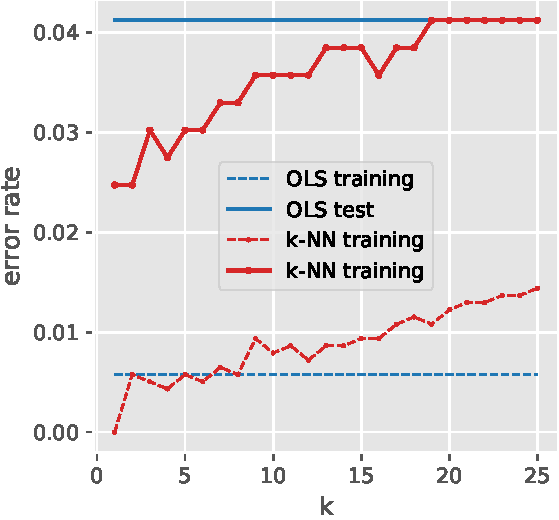
\includegraphics[width=\half]{E2p8_A.pdf}
\end{minipage}\halfspace
\begin{minipage}{\half}
\centering
\begin{tabular}{|c|c|c|}
\hline
\textbf{Model} & \textbf{Training error} & \textbf{Test error}\\
\hline
OLS & 0.58 \% & 4.12 \% \\
\hline
1-NN & 0 & 2.47 \% \\
\hline
3-NN & 0.50 \% & 3.02 \% \\
\hline
5-NN & 0.58 \% & 3.02 \% \\
\hline
7-NN & 0.65 \% & 3.30 \% \\
\hline
15-NN & 0.94 \% & 3.85 \% \\
\hline
\end{tabular}
\end{minipage}



\subsection*{Ex. 2.9}
Let's denote $R(Z_{tr}, Z_{te})$ the average of squared residuals for $Z_{te}$ using the OLS coefficients from $Z_{tr}$. Using the notation from the exercise:
\begin{eqnarray*}
R_{tr}(\hat{\beta}) \equiv R(Z_{tr}, Z_{tr}), \qquad R_{te}(\hat{\beta}) \equiv R(Z_{tr}, Z_{te})
\end{eqnarray*}
It is easy to verify that the expected value $ \mathbb{E}_{Z_{te}} \left[ R(Z_{tr}, Z_{te}) \right]$ does not depend on $M \equiv |Z_{te}|$ (assuming the test examples are i.i.d.). This allows us to take $M = N$. Now, by definition of OLS estimates we have:
\begin{eqnarray*}
R(Z_{te}, Z_{te}) \leq R(Z_{tr}, Z_{te})
\end{eqnarray*}
Now that $M = N$, the lhs has the same distribution as $R(Z_{tr}, Z_{tr})$, so when taking the expectation value:
\begin{eqnarray*}
\mathbb{E}_{Z_{te}, Z_{tr}} \left[ R(Z_{tr}, Z_{tr}) \right] = \mathbb{E}_{Z_{te}, Z_{tr}} \left[ R(Z_{te}, Z_{te}) \right] \leq \mathbb{E}_{Z_{te}, Z_{tr}} \left[ R(Z_{tr}, Z_{te})  \right]
\end{eqnarray*}
which proves the assertion.